\section{Experiments}

\begin{figure*}
\begin{center}
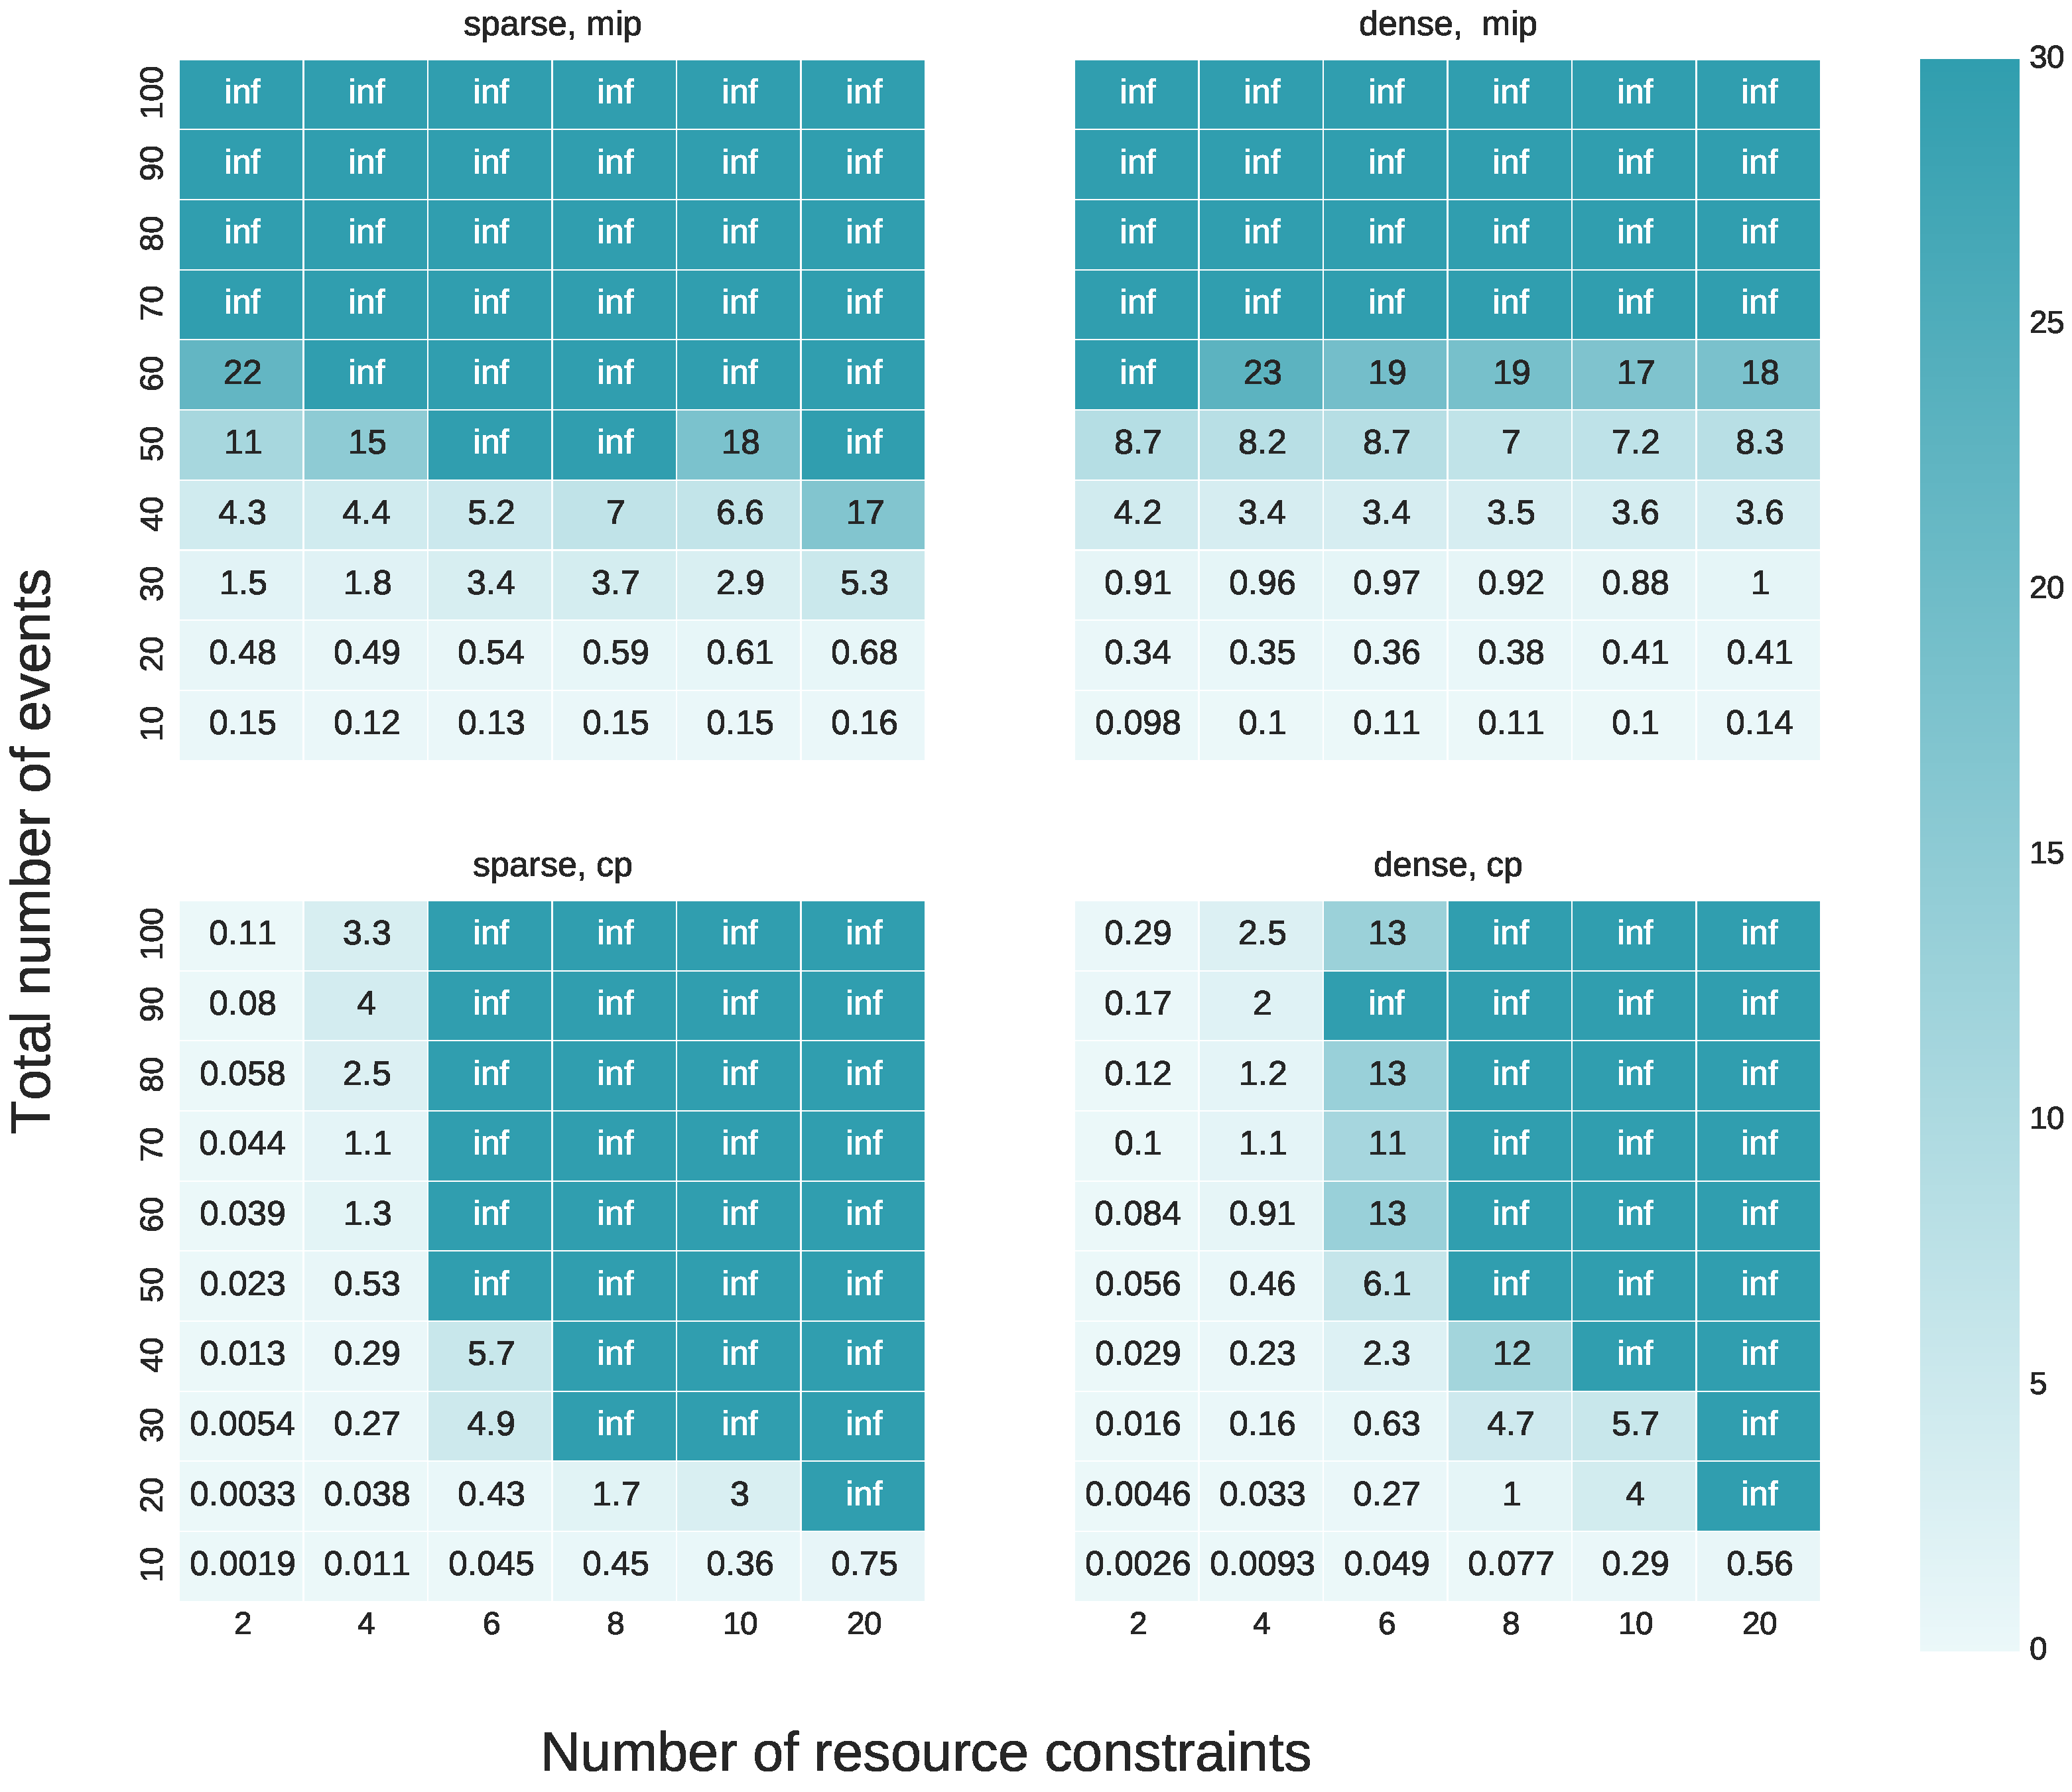
\includegraphics[width=\textwidth]{execution_time}
\caption{Comporison of execution time for different types of networks, or \texttt{inf} if the solver failed to compute the result within time limit. Y axis represents the number of nodes in the temporal network ($N$). X axis represents the number of resource constraints ($R$). Top portion of the figure was obtained using the MIP-based solver, while bottom part of the figure was obtained using CSP-based solver. The left side of the figure represents computations on \textit{sparse} networks, which in this case means that the total number of temporal constraints is $2N$. On the right side we have \textit{dense} networks, meaning that the number of temporal constraints is $N^2/2$.}
\label{fig:execution_time}
\end{center}
\end{figure*}

\begin{figure*}
\begin{center}
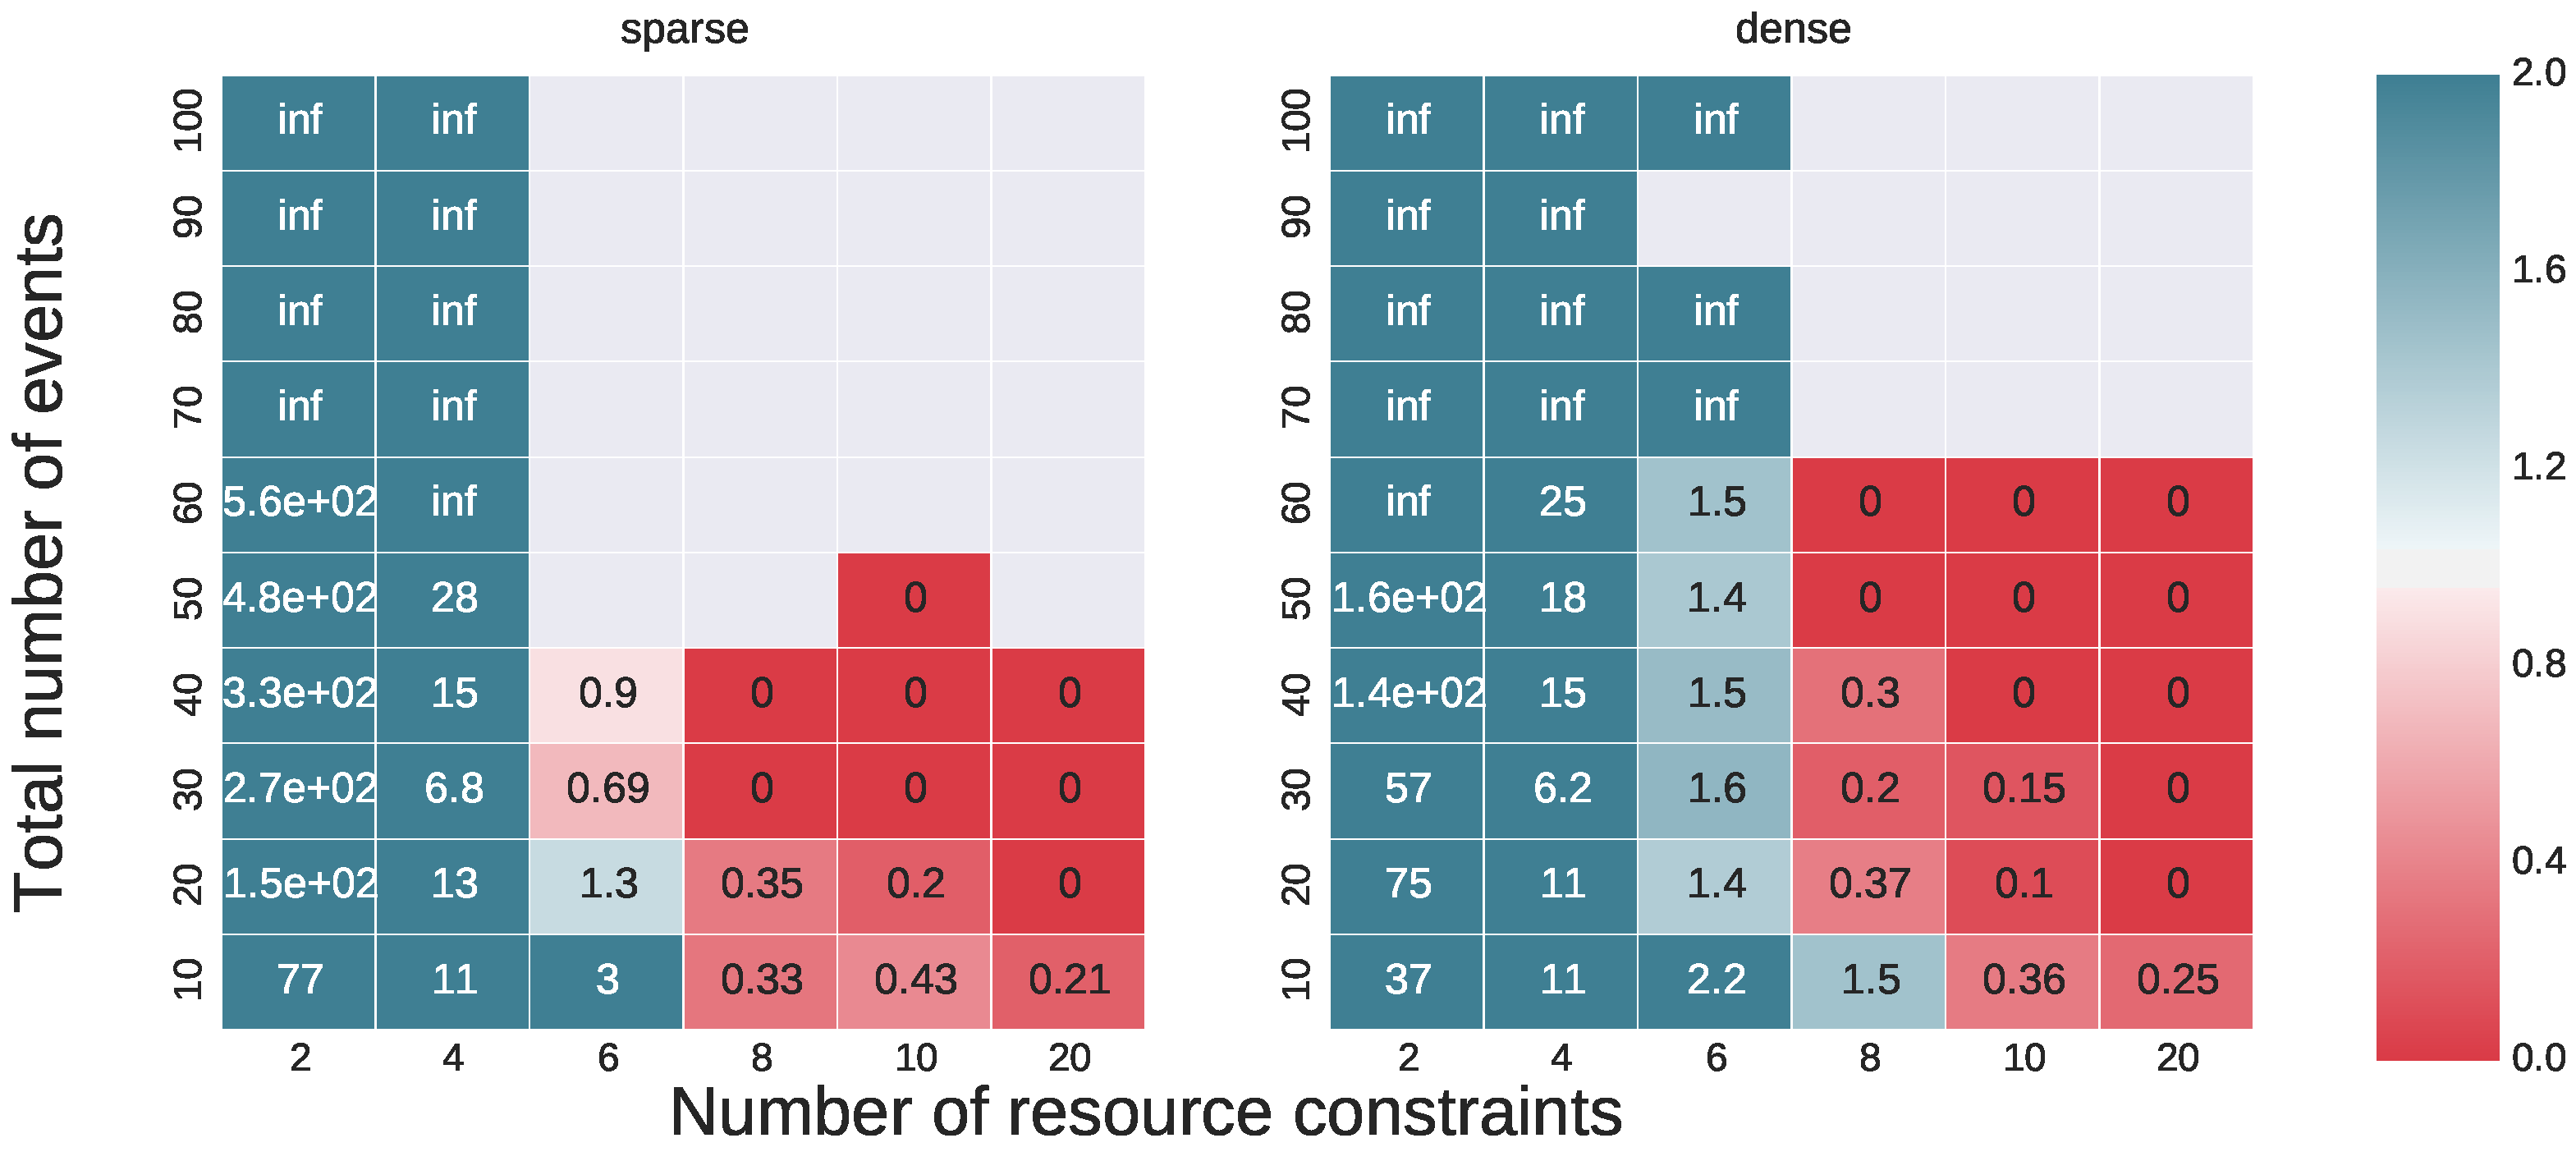
\includegraphics[width=\textwidth]{when_better}
\caption{Number on the figure represents execution time using MIP-based algorithm divided by execution time using CSP-based algorithm. Notice that in particular $0$, means that CSP-based algorithm failed to compute the results within the time limit and \texttt{inf} means that MIP-based algorithm timed out. The missing cells correspond to the networks where both of the algorithms timed out and therefore their execution time cannot be compared.   }
\label{fig:when_better}
\end{center}
\end{figure*}

\subsection{TRN over STN}
To compare both algorithms we chose a simple example of TRN over STN. In case of MIP based algorithm all the temporal constraints $l \leq x - y \leq u$, where $l,b \in \mathbb{R}$ and $x,y \in nodes(ATN)$ can be expressed as simple linear constraints, with $x$ and $y$ being continuous variables. In case of CSP based algorithm we used Floyd-Warshall to determine temporal consistency as suggested in \cite{dechter1991temporal}. The test cases were created by the following procedure:
\begin{enumerate}
\item Specify number of nodes $N \geq 2$, number of temporal constraints $T\geq 2$ and number of resource constraints $R\geq 2$
\item Create a random schedule $s$ for nodes in $N$ with times in the interval $(0.0, 1.0)$.
\item Create $T$ time constraints using the following procedure:
  \begin{enumerate}
  \item Choose start and end points $x,y \in N$.
  \item Choose a type of constraint - lower bound or upper bound, each with probability $0.5$
  \item Let $d=s(y) - s(x)$ and chose number $d'$ form exponential distribution with $\lambda = 1 / \sqrt{d}$. For lower-bound set $l = d - d'$. For upper bound set $u = d + d'$.
  \end{enumerate}
\item Choose number of generating constraints $G$ as a random integer between $1$ and $R-1$ and set number of consuming constraints as $C = R - G$ (so that there's at least on constraint of each type).
\item Create $G$ generating constraints using the following procedure, by randomly choosing $x,y \in N$ and setting $r$ to a random number between $-1 and 0$.
\item Create $C$ consuming constraints using the following procedure.
  \begin{enumerate}
  \item Choose start and end points $x,y \in N$.
  \item Let $m$ be the maximum resource usage value between $x$ and $y$ considering all the resource constraints generated so far. If $m = 0$ repeat the process.
  \item choose $r$ from uniform distribution between $0$ and $-m$.
  \end{enumerate}
\end{enumerate}

We considered $10$ different values of $N$: $10, 20, ..., 100$. We considered $6$ different values of $R$: $2, 4, 6, 8, 10, 20$. To chose $T$ we defined two types of networks - sparse, where $T = 2N$ and dense where $T = N^2/2$. For every set of parameters we run $15$ trials. We set the time limit to $30$ seconds. The results are presented on figure \ref{fig:execution_time}. We can see there exist set of parameters where only CSP managed to find the solution MIP exceed the time limit and vice versa. Figure \ref{fig:when_better} compares execution time of CP and MIP algorithms. The cells colored in blue are the ones where CSP algorithm is faster and the cells colored in red are the ones where MIP based algorithm is better. One can see that CSP is much better suited for large temporal networks with small number of resource constraints, while MIP scales much better with the number of resource constraints.




\subsection{TRN over pSTN}
To demonstrate extensibility of our approach we have implemented a version of TRN network, where the underlying temporal network is pSTN (\cite{Fang2014}). pSTN extends the notion of STN. For this discussion we define STN nodes and edges as \textbf{actiavated time points} and \textbf{free constraints} respectively. pSTN defines \textbf{received time point} which is determined by the environment. Every received time point is defined by corresponding \textbf{uncertain duration (uDn)} constraint, which specifies a probability distribution over duration between an activated time point and a received time point. Due to that extension, the notion of consistency becomes probabilistic; rather than asking \textit{is this pSTN consistent?}, we ask is \textit{is this pSTN consistent with probability $p$?}. Since pSTN is an extension of STN, it is an ATN.

Let's consider the following Smart House scenario. We have $150W$ generator which is available. We know that the user comes back from work at some time defined by a gaussian distribution $N(5pm, 5m)$. Moreover we know that sun sets at time defined by $N(7pm, 1m)$. We would like to meet the following constraints with the overall probability at least $98\%$:
\begin{itemize}
\item Wash clothes (duration: $2h$, power usage: $130W$) before user comes back from work
\item Cook dinner (duration: $30m$, power usage: $100W$) ready within 15 minutes of user coming back from work
\item Have the lights on (power usage: $80W$) from before sunset to at least midnight.
\item Cook a late night snack (duration: $30m$, power usage: $20W$) between 10pm and 11pm.
\end{itemize}


\begin{figure}[H]
\begin{center}
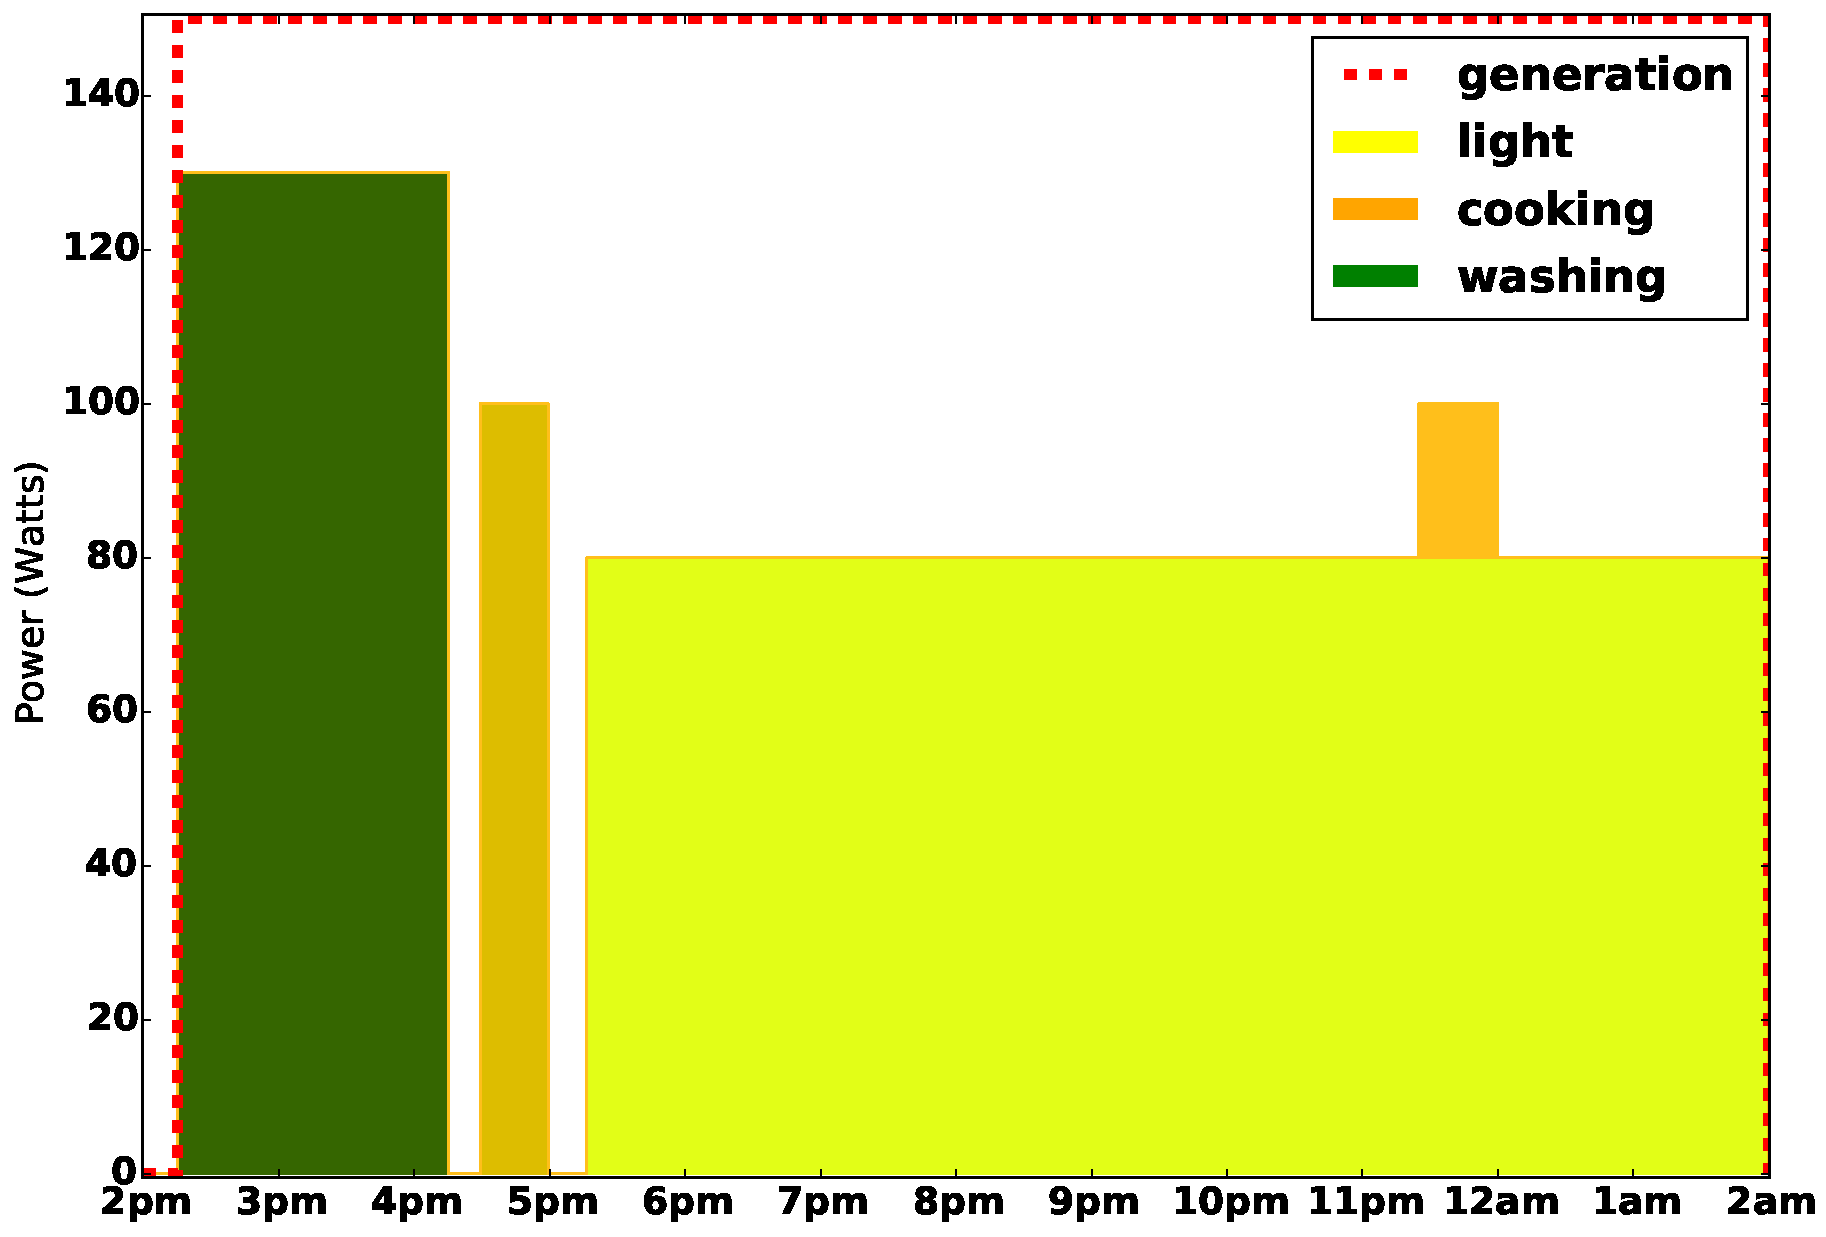
\includegraphics[width=0.49\textwidth]{pstnu_scheduling}
\caption{Depiction of solution to TRN spanning a pSTN.}
\label{fig:pstnu_scheduling}
\end{center}
\end{figure}

Our algorithm successfully finds a solution to this scenario which meets the constraints with probability $99,7\%$, which is more than required. It is presented on fig. \ref{fig:pstnu_scheduling}.
